As explained in last experiment, deletion of Rc has significant overhead than normal reference. 
By learning this result, our assumption here is that deletion of Arc has also overhead when we compare to normal reference. 
In many situation where developer writes a multithreading code, Arc is used and the deletion happens multiple times. 
To assess runtime overhead of algorithm with Arc, We implement merge-sort algorithm in two different ways. 
One is sharing source vector with Arc. The other is passing reference of source vector to child thread. 

Our merge-sort algorithms are implemented with recursion. For each call of recursive function, 
Arc or slice of the source vector needs to be passed and deleted when the function returns value. 
These merge-sort algorithms trigger large number of Arc or reference deletion proportional to the number of call recursive function.
Merge-sort algorithm can be separated in three phases: splitting phase, copying phase, and merging phase. 

The splitting phase is merely acquiring index of range. At this phase, multiple threads are generated and Arc or reference of source vector are passed by calling recursive function. 
Copying phase occurs in the base case of the recursive call. The element in the source vector in a certain index is deep-copied into newly allocated vector.
At merge phase, merge function receives two sorted independent vector and merge them into single new vector.

We use scope method from crossbeam crate to perform multithread programming. 
Scoped thread can have reference to value from its parent thread by ensuring children threads are joined before their parent thread returns value. 
By using scoped thread, we can implement two merge-sort algorithms in identical way except whether the function receives Arc or reference of source vector.
The representations of source vector for each algorithm are shown in Figure~\ref{fig:source_merge_sort}.
The elements of source vector are CustomerOwned objects. We generates source vectors in size of 4, 8, 12 and 16 million.
Finally, merge-sort is performed based on value of key field. The figure shows the result for runtime performance of merge-sort algorithms on difference size of vectors. 

\begin{figure}[htb]
    \begin{lstlisting}
        // Source vector for algorithm with Arc.
        arr: Arc<VecDeque<T>>

        // Source vector for algorithm with reference (slice).
        arr: &[T]
    \end{lstlisting}
    \caption{Representation of Source Vector}
    \label{fig:source_merge_sort}
\end{figure}


\subsection{Result}
Figure~\ref{fig:source_merge_sort} shows the runtime performance of our merge-sort algorithm with specified Vec sizes. 
The blue and yellow bar charts represent the runtime performance of merge-sort algorithm using reference and Arc respectively. 
The result says that algorithms with Arc is about 21\% slower than algorithms with reference.

\begin{figure}[htb]
    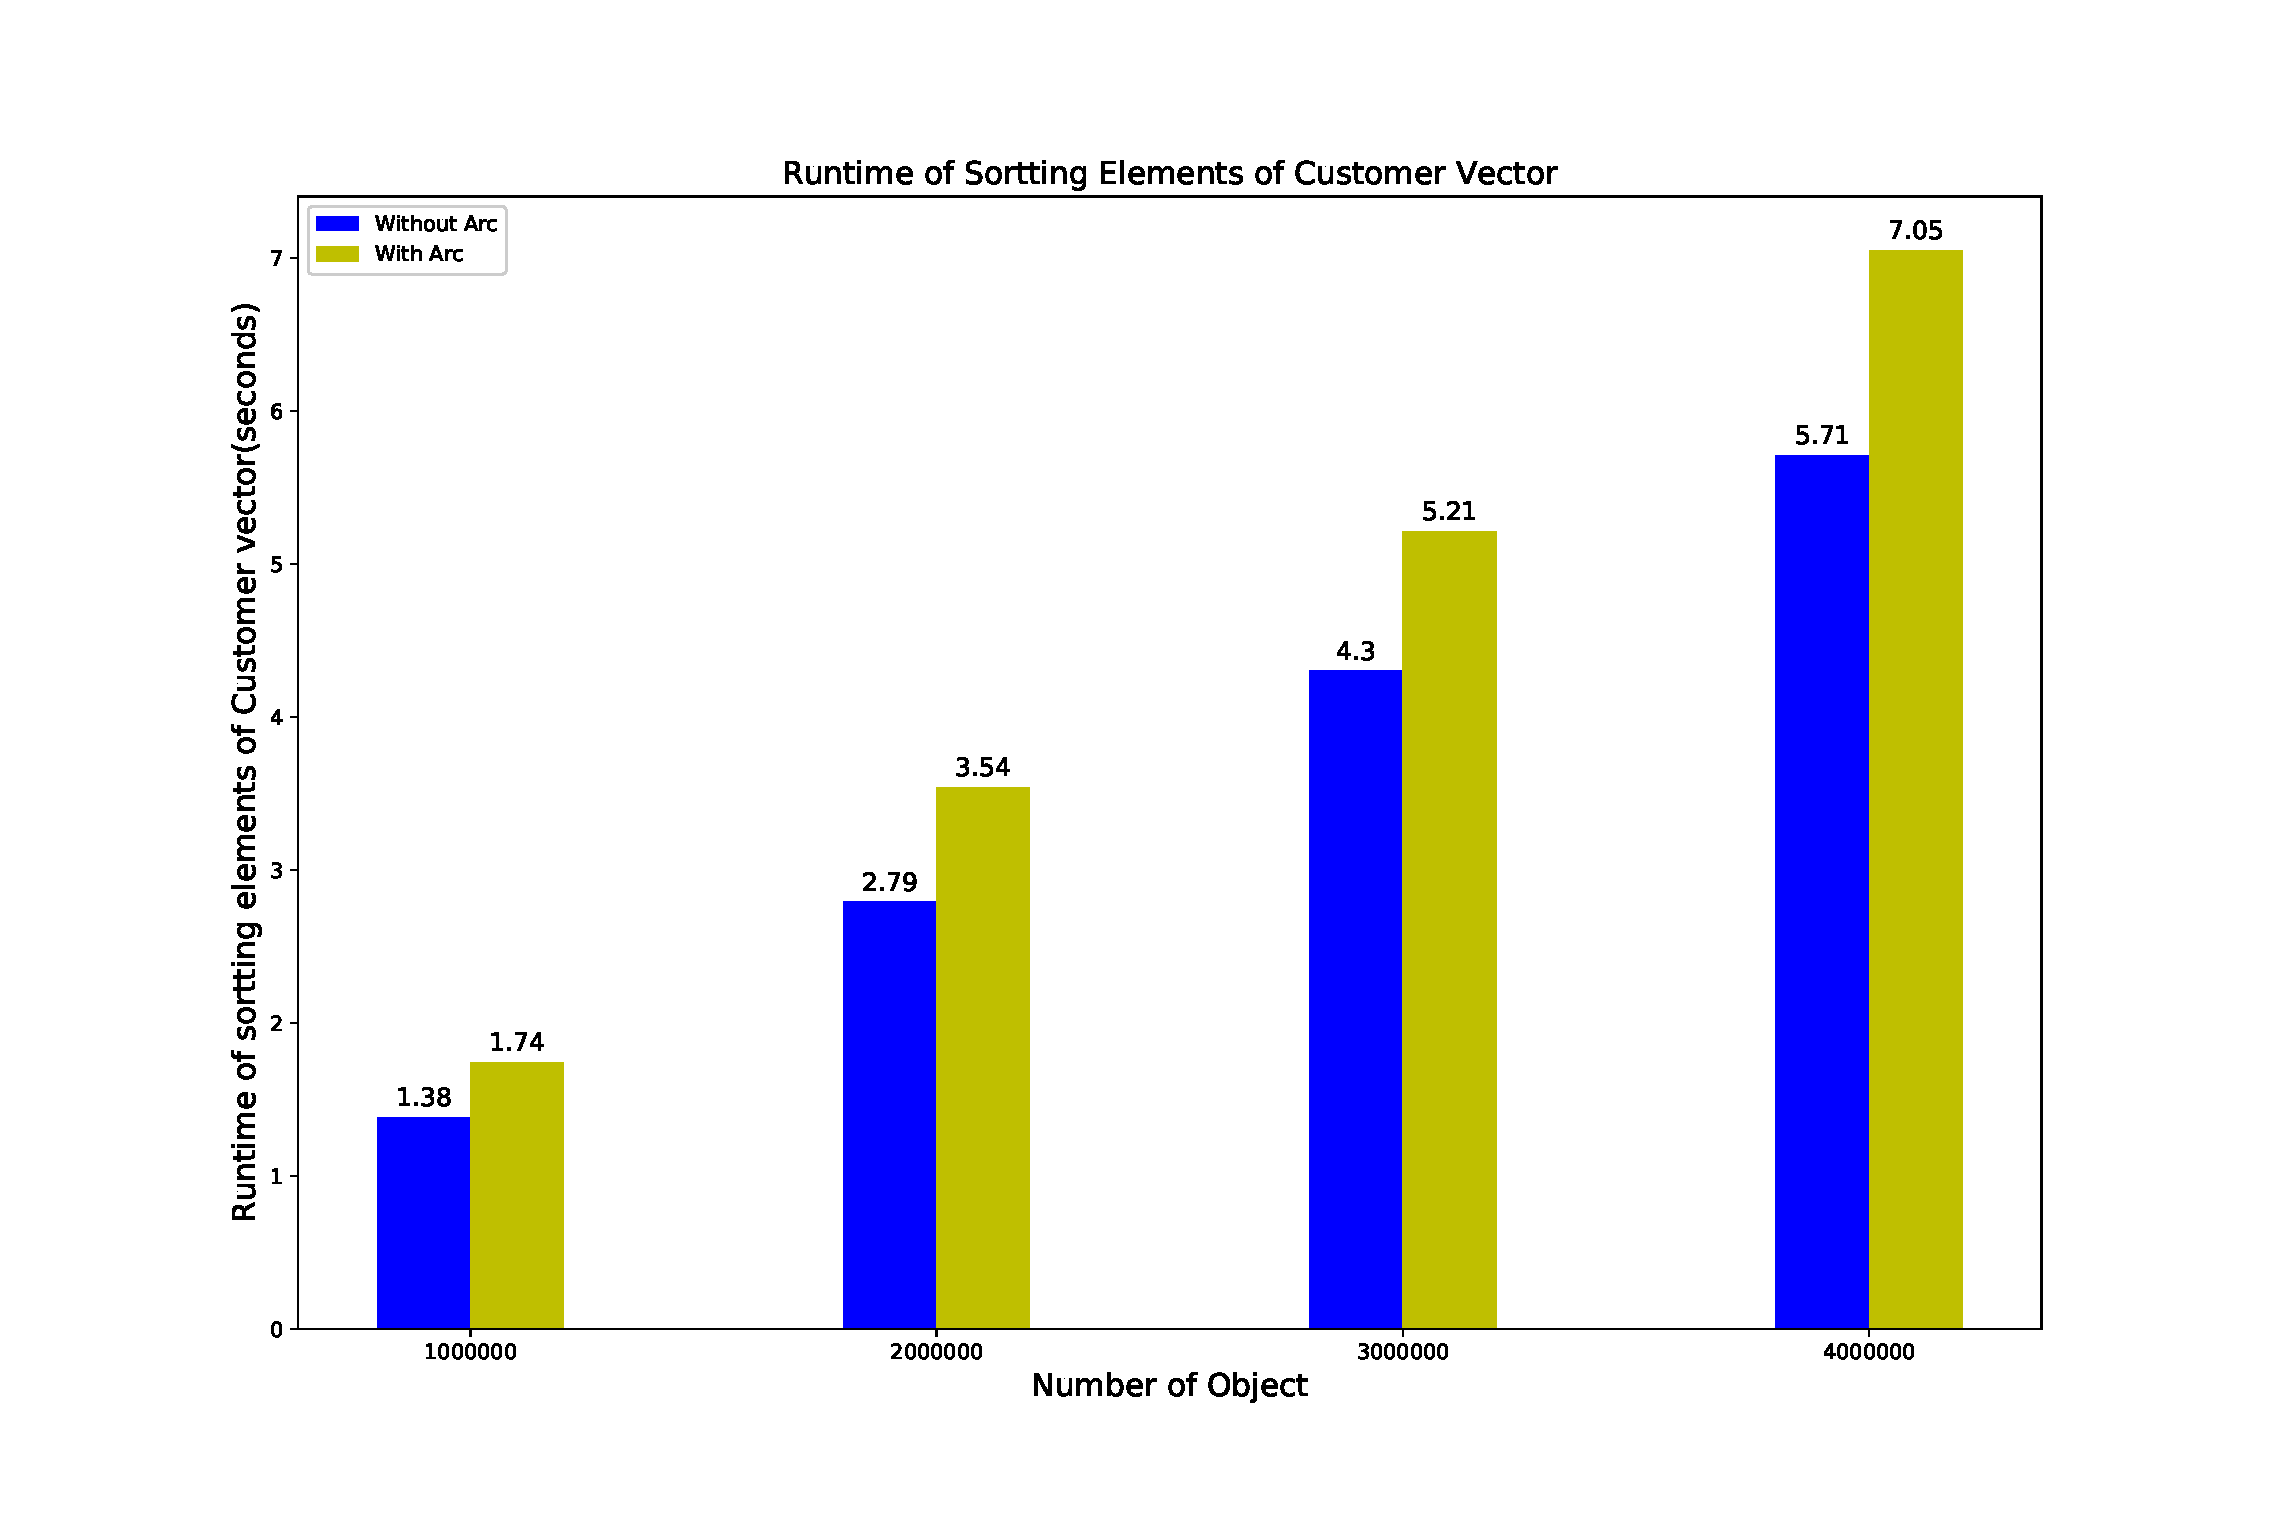
\includegraphics[width=15cm]{rust_merge_sort.eps}
    \caption{Runtime of Sorting Elements of Customer Vector}
    \label{fig:merge_sort}
\end{figure}

\subsection{Discussion}
The reason why merge-sort algorithm with Arc is much slower than one with reference is 
the same for the reason why dropping Rc shows overhead compared to dropping reference.
Arc has to check the number of variable pointing to the actual content and decide 
deallocate the memory or not.

In addition, Arc uses atomic operations for tis reference counting. Atomic operations bring thread-safety, but they are more expensive than ordinary memory accesses.
Therefore, when sharing reference counting between threads is not required, using Rc is the recommended way \cite{RustArcPage}.

In the situation like our experiment, normal reference can be used instead of Arc to share data between threads. 
This solution results in better runtime performance in our experiment. Therefore, one should use reference to share data among different threads 
whenever it is possible.

